\documentclass[twoside]{book}

% Packages required by doxygen
\usepackage{fixltx2e}
\usepackage{calc}
\usepackage{doxygen}
\usepackage[export]{adjustbox} % also loads graphicx
\usepackage{graphicx}
\usepackage[utf8]{inputenc}
\usepackage{makeidx}
\usepackage{multicol}
\usepackage{multirow}
\PassOptionsToPackage{warn}{textcomp}
\usepackage{textcomp}
\usepackage[nointegrals]{wasysym}
\usepackage[table]{xcolor}

% Font selection
\usepackage[T1]{fontenc}
\usepackage[scaled=.90]{helvet}
\usepackage{courier}
\usepackage{amssymb}
\usepackage{sectsty}
\renewcommand{\familydefault}{\sfdefault}
\allsectionsfont{%
  \fontseries{bc}\selectfont%
  \color{darkgray}%
}
\renewcommand{\DoxyLabelFont}{%
  \fontseries{bc}\selectfont%
  \color{darkgray}%
}
\newcommand{\+}{\discretionary{\mbox{\scriptsize$\hookleftarrow$}}{}{}}

% Page & text layout
\usepackage{geometry}
\geometry{%
  a4paper,%
  top=2.5cm,%
  bottom=2.5cm,%
  left=2.5cm,%
  right=2.5cm%
}
\tolerance=750
\hfuzz=15pt
\hbadness=750
\setlength{\emergencystretch}{15pt}
\setlength{\parindent}{0cm}
\setlength{\parskip}{3ex plus 2ex minus 2ex}
\makeatletter
\renewcommand{\paragraph}{%
  \@startsection{paragraph}{4}{0ex}{-1.0ex}{1.0ex}{%
    \normalfont\normalsize\bfseries\SS@parafont%
  }%
}
\renewcommand{\subparagraph}{%
  \@startsection{subparagraph}{5}{0ex}{-1.0ex}{1.0ex}{%
    \normalfont\normalsize\bfseries\SS@subparafont%
  }%
}
\makeatother

% Headers & footers
\usepackage{fancyhdr}
\pagestyle{fancyplain}
\fancyhead[LE]{\fancyplain{}{\bfseries\thepage}}
\fancyhead[CE]{\fancyplain{}{}}
\fancyhead[RE]{\fancyplain{}{\bfseries\leftmark}}
\fancyhead[LO]{\fancyplain{}{\bfseries\rightmark}}
\fancyhead[CO]{\fancyplain{}{}}
\fancyhead[RO]{\fancyplain{}{\bfseries\thepage}}
\fancyfoot[LE]{\fancyplain{}{}}
\fancyfoot[CE]{\fancyplain{}{}}
\fancyfoot[RE]{\fancyplain{}{\bfseries\scriptsize Generated by Doxygen }}
\fancyfoot[LO]{\fancyplain{}{\bfseries\scriptsize Generated by Doxygen }}
\fancyfoot[CO]{\fancyplain{}{}}
\fancyfoot[RO]{\fancyplain{}{}}
\renewcommand{\footrulewidth}{0.4pt}
\renewcommand{\chaptermark}[1]{%
  \markboth{#1}{}%
}
\renewcommand{\sectionmark}[1]{%
  \markright{\thesection\ #1}%
}

% Indices & bibliography
\usepackage{natbib}
\usepackage[titles]{tocloft}
\setcounter{tocdepth}{3}
\setcounter{secnumdepth}{5}
\makeindex

% Hyperlinks (required, but should be loaded last)
\usepackage{ifpdf}
\ifpdf
  \usepackage[pdftex,pagebackref=true]{hyperref}
\else
  \usepackage[ps2pdf,pagebackref=true]{hyperref}
\fi
\hypersetup{%
  colorlinks=true,%
  linkcolor=blue,%
  citecolor=blue,%
  unicode%
}

% Custom commands
\newcommand{\clearemptydoublepage}{%
  \newpage{\pagestyle{empty}\cleardoublepage}%
}

\usepackage{caption}
\captionsetup{labelsep=space,justification=centering,font={bf},singlelinecheck=off,skip=4pt,position=top}

%===== C O N T E N T S =====

\begin{document}

% Titlepage & ToC
\hypersetup{pageanchor=false,
             bookmarksnumbered=true,
             pdfencoding=unicode
            }
\pagenumbering{alph}
\begin{titlepage}
\vspace*{7cm}
\begin{center}%
{\Large Snake Projekt }\\
\vspace*{1cm}
{\large Generated by Doxygen 1.8.14}\\
\end{center}
\end{titlepage}
\clearemptydoublepage
\pagenumbering{roman}
\tableofcontents
\clearemptydoublepage
\pagenumbering{arabic}
\hypersetup{pageanchor=true}

%--- Begin generated contents ---
\chapter{Namespace Index}
\section{Namespace List}
Here is a list of all namespaces with brief descriptions\+:\begin{DoxyCompactList}
\item\contentsline{section}{\mbox{\hyperlink{namespace_snake_01_projekt_01auf_01_python}{Snake Projekt auf Python}} }{\pageref{namespace_snake_01_projekt_01auf_01_python}}{}
\end{DoxyCompactList}

\chapter{Hierarchical Index}
\section{Class Hierarchy}
This inheritance list is sorted roughly, but not completely, alphabetically\+:\begin{DoxyCompactList}
\item Frame\begin{DoxyCompactList}
\item \contentsline{section}{Snake\+\_\+spiel}{\pageref{class_snake_01_projekt_01auf_01_python_1_1_snake__spiel}}{}
\end{DoxyCompactList}
\item object\begin{DoxyCompactList}
\item \contentsline{section}{Arduino}{\pageref{class_snake_01_projekt_01auf_01_python_1_1_arduino}}{}
\end{DoxyCompactList}
\item \contentsline{section}{Snake}{\pageref{class_snake_01_projekt_01auf_01_python_1_1_snake}}{}
\item \contentsline{section}{Snake\+Körper\+Stück}{\pageref{class_snake_01_projekt_01auf_01_python_1_1_snake_k_xC3_xB6rper_st_xC3_xBCck}}{}
\item Stream\begin{DoxyCompactList}
\item \contentsline{section}{Esp\+Server}{\pageref{class_esp_server}}{}
\end{DoxyCompactList}
\item \contentsline{section}{Welt}{\pageref{class_snake_01_projekt_01auf_01_python_1_1_welt}}{}
\end{DoxyCompactList}

\chapter{Data Structure Index}
\section{Data Structures}
Here are the data structures with brief descriptions\+:\begin{DoxyCompactList}
\item\contentsline{section}{\mbox{\hyperlink{class_snake_01_projekt_01auf_01_python_1_1_arduino}{Arduino}} }{\pageref{class_snake_01_projekt_01auf_01_python_1_1_arduino}}{}
\item\contentsline{section}{\mbox{\hyperlink{class_esp_server}{Esp\+Server}} }{\pageref{class_esp_server}}{}
\item\contentsline{section}{\mbox{\hyperlink{class_snake_01_projekt_01auf_01_python_1_1_snake}{Snake}} }{\pageref{class_snake_01_projekt_01auf_01_python_1_1_snake}}{}
\item\contentsline{section}{\mbox{\hyperlink{class_snake_01_projekt_01auf_01_python_1_1_snake__spiel}{Snake\+\_\+spiel}} }{\pageref{class_snake_01_projekt_01auf_01_python_1_1_snake__spiel}}{}
\item\contentsline{section}{\mbox{\hyperlink{class_snake_01_projekt_01auf_01_python_1_1_snake_k_xC3_xB6rper_st_xC3_xBCck}{Snake\+Körper\+Stück}} }{\pageref{class_snake_01_projekt_01auf_01_python_1_1_snake_k_xC3_xB6rper_st_xC3_xBCck}}{}
\item\contentsline{section}{\mbox{\hyperlink{class_snake_01_projekt_01auf_01_python_1_1_welt}{Welt}} }{\pageref{class_snake_01_projekt_01auf_01_python_1_1_welt}}{}
\end{DoxyCompactList}

\chapter{File Index}
\section{File List}
Here is a list of all files with brief descriptions\+:\begin{DoxyCompactList}
\item\contentsline{section}{C\+:/\+Users/soere/\+Desktop/\+Projekt Snake/\mbox{\hyperlink{_snake_01_projekt_01auf_01_python_8py}{Snake Projekt auf Python.\+py}} }{\pageref{_snake_01_projekt_01auf_01_python_8py}}{}
\item\contentsline{section}{C\+:/\+Users/soere/\+Desktop/\+Projekt Snake/\+Projekt\+\_\+\+Snake/\mbox{\hyperlink{_dumb_server_8cpp}{Dumb\+Server.\+cpp}} }{\pageref{_dumb_server_8cpp}}{}
\item\contentsline{section}{C\+:/\+Users/soere/\+Desktop/\+Projekt Snake/\+Projekt\+\_\+\+Snake/\mbox{\hyperlink{_dumb_server_8h}{Dumb\+Server.\+h}} }{\pageref{_dumb_server_8h}}{}
\end{DoxyCompactList}

\chapter{Namespace Documentation}
\hypertarget{namespace_snake_01_projekt_01auf_01_python}{}\section{Snake Projekt auf Python Namespace Reference}
\label{namespace_snake_01_projekt_01auf_01_python}\index{Snake Projekt auf Python@{Snake Projekt auf Python}}
\subsection*{Data Structures}
\begin{DoxyCompactItemize}
\item 
class \mbox{\hyperlink{class_snake_01_projekt_01auf_01_python_1_1_arduino}{Arduino}}
\item 
class \mbox{\hyperlink{class_snake_01_projekt_01auf_01_python_1_1_snake}{Snake}}
\item 
class \mbox{\hyperlink{class_snake_01_projekt_01auf_01_python_1_1_snake__spiel}{Snake\+\_\+spiel}}
\item 
class \mbox{\hyperlink{class_snake_01_projekt_01auf_01_python_1_1_snake_k_xC3_xB6rper_st_xC3_xBCck}{Snake\+Körper\+Stück}}
\item 
class \mbox{\hyperlink{class_snake_01_projekt_01auf_01_python_1_1_welt}{Welt}}
\end{DoxyCompactItemize}
\subsection*{Variables}
\begin{DoxyCompactItemize}
\item 
int \mbox{\hyperlink{namespace_snake_01_projekt_01auf_01_python_a0bb194ef42a009e15b75b9c78234ec82}{W\+E\+L\+T\+\_\+\+G\+RÖ\+S\+SE}} = 500 \char`\"{}\char`\"{}\char`\"{}Allgemeine Spiel Infos\char`\"{}\char`\"{}\char`\"{}
\item 
int \mbox{\hyperlink{namespace_snake_01_projekt_01auf_01_python_a0490a870a678eec59b0e01ade54e7cf5}{Z\+E\+L\+L\+EN}} = 8
\item 
int \mbox{\hyperlink{namespace_snake_01_projekt_01auf_01_python_abfd2595e2773b407f4e4d36545e0d6c2}{S\+N\+A\+K\+E\+T\+E\+M\+PO}} = 200
\item 
\mbox{\hyperlink{namespace_snake_01_projekt_01auf_01_python_a494a6a834239a0d8becd8a87a00ec956}{V\+E\+R\+B\+I\+N\+D\+EN}} = int(input(\char`\"{}Mit \mbox{\hyperlink{class_snake_01_projekt_01auf_01_python_1_1_arduino}{Arduino}} verbinden? Ja(1) Nein(0)\char`\"{}))
\item 
\mbox{\hyperlink{namespace_snake_01_projekt_01auf_01_python_aa798779259654cac04213978cf4297ab}{snake}} = \mbox{\hyperlink{class_snake_01_projekt_01auf_01_python_1_1_snake}{Snake}}()
\item 
\mbox{\hyperlink{namespace_snake_01_projekt_01auf_01_python_a80417409ca56d97eabc593c02dbb4a1c}{welt}} = \mbox{\hyperlink{class_snake_01_projekt_01auf_01_python_1_1_welt}{Welt}}(\mbox{\hyperlink{namespace_snake_01_projekt_01auf_01_python_aa798779259654cac04213978cf4297ab}{snake}})
\item 
\mbox{\hyperlink{namespace_snake_01_projekt_01auf_01_python_a21846080f3e252e582ecd7bf21d38f90}{spiel}} = \mbox{\hyperlink{class_snake_01_projekt_01auf_01_python_1_1_snake__spiel}{Snake\+\_\+spiel}}(\mbox{\hyperlink{namespace_snake_01_projekt_01auf_01_python_a80417409ca56d97eabc593c02dbb4a1c}{welt}}, \mbox{\hyperlink{namespace_snake_01_projekt_01auf_01_python_aa798779259654cac04213978cf4297ab}{snake}})
\item 
\mbox{\hyperlink{namespace_snake_01_projekt_01auf_01_python_a9a3afecebf45ad60fdcaa433890500d8}{canv}} = Canvas(spiel.\+master, width=\mbox{\hyperlink{namespace_snake_01_projekt_01auf_01_python_a0bb194ef42a009e15b75b9c78234ec82}{W\+E\+L\+T\+\_\+\+G\+RÖ\+S\+SE}}, height=\mbox{\hyperlink{namespace_snake_01_projekt_01auf_01_python_a0bb194ef42a009e15b75b9c78234ec82}{W\+E\+L\+T\+\_\+\+G\+RÖ\+S\+SE}})
\end{DoxyCompactItemize}


\subsection{Variable Documentation}
\mbox{\Hypertarget{namespace_snake_01_projekt_01auf_01_python_a9a3afecebf45ad60fdcaa433890500d8}\label{namespace_snake_01_projekt_01auf_01_python_a9a3afecebf45ad60fdcaa433890500d8}} 
\index{Snake Projekt auf Python@{Snake Projekt auf Python}!canv@{canv}}
\index{canv@{canv}!Snake Projekt auf Python@{Snake Projekt auf Python}}
\subsubsection{\texorpdfstring{canv}{canv}}
{\footnotesize\ttfamily canv = Canvas(spiel.\+master, width=\mbox{\hyperlink{namespace_snake_01_projekt_01auf_01_python_a0bb194ef42a009e15b75b9c78234ec82}{W\+E\+L\+T\+\_\+\+G\+RÖ\+S\+SE}}, height=\mbox{\hyperlink{namespace_snake_01_projekt_01auf_01_python_a0bb194ef42a009e15b75b9c78234ec82}{W\+E\+L\+T\+\_\+\+G\+RÖ\+S\+SE}})}

\mbox{\Hypertarget{namespace_snake_01_projekt_01auf_01_python_aa798779259654cac04213978cf4297ab}\label{namespace_snake_01_projekt_01auf_01_python_aa798779259654cac04213978cf4297ab}} 
\index{Snake Projekt auf Python@{Snake Projekt auf Python}!snake@{snake}}
\index{snake@{snake}!Snake Projekt auf Python@{Snake Projekt auf Python}}
\subsubsection{\texorpdfstring{snake}{snake}}
{\footnotesize\ttfamily snake = \mbox{\hyperlink{class_snake_01_projekt_01auf_01_python_1_1_snake}{Snake}}()}

\mbox{\Hypertarget{namespace_snake_01_projekt_01auf_01_python_abfd2595e2773b407f4e4d36545e0d6c2}\label{namespace_snake_01_projekt_01auf_01_python_abfd2595e2773b407f4e4d36545e0d6c2}} 
\index{Snake Projekt auf Python@{Snake Projekt auf Python}!S\+N\+A\+K\+E\+T\+E\+M\+PO@{S\+N\+A\+K\+E\+T\+E\+M\+PO}}
\index{S\+N\+A\+K\+E\+T\+E\+M\+PO@{S\+N\+A\+K\+E\+T\+E\+M\+PO}!Snake Projekt auf Python@{Snake Projekt auf Python}}
\subsubsection{\texorpdfstring{S\+N\+A\+K\+E\+T\+E\+M\+PO}{SNAKETEMPO}}
{\footnotesize\ttfamily int S\+N\+A\+K\+E\+T\+E\+M\+PO = 200}

\mbox{\Hypertarget{namespace_snake_01_projekt_01auf_01_python_a21846080f3e252e582ecd7bf21d38f90}\label{namespace_snake_01_projekt_01auf_01_python_a21846080f3e252e582ecd7bf21d38f90}} 
\index{Snake Projekt auf Python@{Snake Projekt auf Python}!spiel@{spiel}}
\index{spiel@{spiel}!Snake Projekt auf Python@{Snake Projekt auf Python}}
\subsubsection{\texorpdfstring{spiel}{spiel}}
{\footnotesize\ttfamily spiel = \mbox{\hyperlink{class_snake_01_projekt_01auf_01_python_1_1_snake__spiel}{Snake\+\_\+spiel}}(\mbox{\hyperlink{namespace_snake_01_projekt_01auf_01_python_a80417409ca56d97eabc593c02dbb4a1c}{welt}}, \mbox{\hyperlink{namespace_snake_01_projekt_01auf_01_python_aa798779259654cac04213978cf4297ab}{snake}})}

\mbox{\Hypertarget{namespace_snake_01_projekt_01auf_01_python_a494a6a834239a0d8becd8a87a00ec956}\label{namespace_snake_01_projekt_01auf_01_python_a494a6a834239a0d8becd8a87a00ec956}} 
\index{Snake Projekt auf Python@{Snake Projekt auf Python}!V\+E\+R\+B\+I\+N\+D\+EN@{V\+E\+R\+B\+I\+N\+D\+EN}}
\index{V\+E\+R\+B\+I\+N\+D\+EN@{V\+E\+R\+B\+I\+N\+D\+EN}!Snake Projekt auf Python@{Snake Projekt auf Python}}
\subsubsection{\texorpdfstring{V\+E\+R\+B\+I\+N\+D\+EN}{VERBINDEN}}
{\footnotesize\ttfamily V\+E\+R\+B\+I\+N\+D\+EN = int(input(\char`\"{}Mit \mbox{\hyperlink{class_snake_01_projekt_01auf_01_python_1_1_arduino}{Arduino}} verbinden? Ja(1) Nein(0)\char`\"{}))}

\mbox{\Hypertarget{namespace_snake_01_projekt_01auf_01_python_a80417409ca56d97eabc593c02dbb4a1c}\label{namespace_snake_01_projekt_01auf_01_python_a80417409ca56d97eabc593c02dbb4a1c}} 
\index{Snake Projekt auf Python@{Snake Projekt auf Python}!welt@{welt}}
\index{welt@{welt}!Snake Projekt auf Python@{Snake Projekt auf Python}}
\subsubsection{\texorpdfstring{welt}{welt}}
{\footnotesize\ttfamily welt = \mbox{\hyperlink{class_snake_01_projekt_01auf_01_python_1_1_welt}{Welt}}(\mbox{\hyperlink{namespace_snake_01_projekt_01auf_01_python_aa798779259654cac04213978cf4297ab}{snake}})}

\mbox{\Hypertarget{namespace_snake_01_projekt_01auf_01_python_a0bb194ef42a009e15b75b9c78234ec82}\label{namespace_snake_01_projekt_01auf_01_python_a0bb194ef42a009e15b75b9c78234ec82}} 
\index{Snake Projekt auf Python@{Snake Projekt auf Python}!W\+E\+L\+T\+\_\+\+G\+RÖ\+S\+SE@{W\+E\+L\+T\+\_\+\+G\+RÖ\+S\+SE}}
\index{W\+E\+L\+T\+\_\+\+G\+RÖ\+S\+SE@{W\+E\+L\+T\+\_\+\+G\+RÖ\+S\+SE}!Snake Projekt auf Python@{Snake Projekt auf Python}}
\subsubsection{\texorpdfstring{W\+E\+L\+T\+\_\+\+G\+RÖ\+S\+SE}{WELT\_GRÖSSE}}
{\footnotesize\ttfamily int W\+E\+L\+T\+\_\+\+G\+RÖ\+S\+SE = 500 \char`\"{}\char`\"{}\char`\"{}Allgemeine Spiel Infos\char`\"{}\char`\"{}\char`\"{}}

\mbox{\Hypertarget{namespace_snake_01_projekt_01auf_01_python_a0490a870a678eec59b0e01ade54e7cf5}\label{namespace_snake_01_projekt_01auf_01_python_a0490a870a678eec59b0e01ade54e7cf5}} 
\index{Snake Projekt auf Python@{Snake Projekt auf Python}!Z\+E\+L\+L\+EN@{Z\+E\+L\+L\+EN}}
\index{Z\+E\+L\+L\+EN@{Z\+E\+L\+L\+EN}!Snake Projekt auf Python@{Snake Projekt auf Python}}
\subsubsection{\texorpdfstring{Z\+E\+L\+L\+EN}{ZELLEN}}
{\footnotesize\ttfamily int Z\+E\+L\+L\+EN = 8}


\chapter{Data Structure Documentation}
\hypertarget{class_snake_01_projekt_01auf_01_python_1_1_arduino}{}\section{Arduino Class Reference}
\label{class_snake_01_projekt_01auf_01_python_1_1_arduino}\index{Arduino@{Arduino}}
Inheritance diagram for Arduino\+:\begin{figure}[H]
\begin{center}
\leavevmode
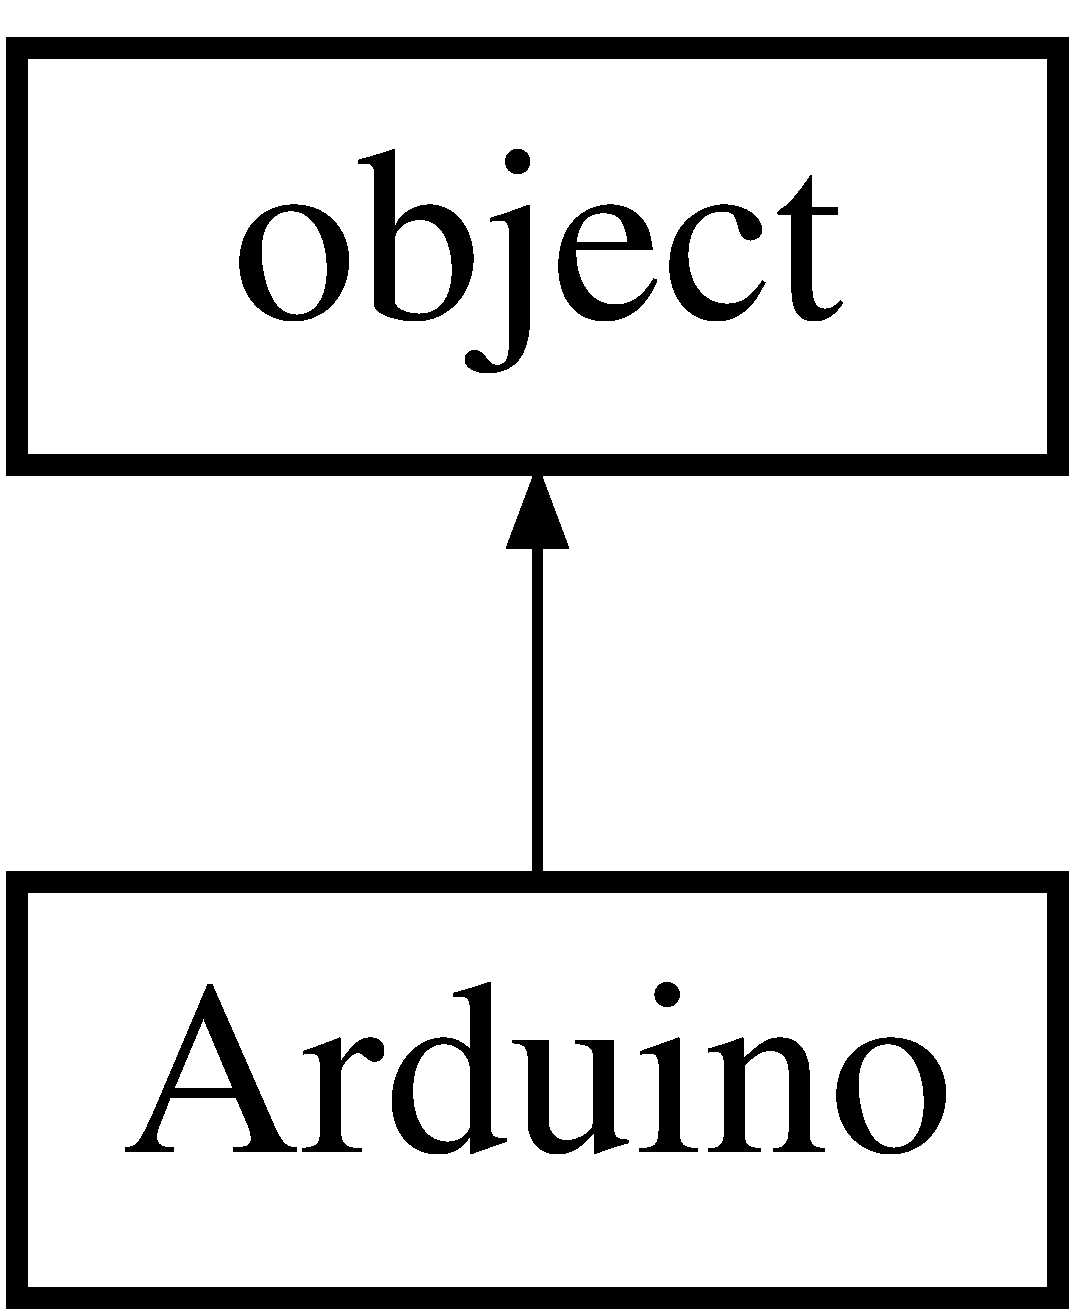
\includegraphics[height=2.000000cm]{class_snake_01_projekt_01auf_01_python_1_1_arduino}
\end{center}
\end{figure}
\subsection*{Public Member Functions}
\begin{DoxyCompactItemize}
\item 
def \mbox{\hyperlink{class_snake_01_projekt_01auf_01_python_1_1_arduino_a3fa102a2756b367e66a90d9f678cd250}{\+\_\+\+\_\+init\+\_\+\+\_\+}} (self, \mbox{\hyperlink{class_snake_01_projekt_01auf_01_python_1_1_arduino_a04a8a2bbfa9c15500892b8e5033d625b}{window}}, host, port)
\item 
def \mbox{\hyperlink{class_snake_01_projekt_01auf_01_python_1_1_arduino_a05097bd2ea4ca3b2c17d7b7164a67539}{send\+\_\+command}} (self, command)
\item 
def \mbox{\hyperlink{class_snake_01_projekt_01auf_01_python_1_1_arduino_a8639372c33e15084a7f7c4d9d87b7bfe}{close}} (self)
\end{DoxyCompactItemize}
\subsection*{Data Fields}
\begin{DoxyCompactItemize}
\item 
\mbox{\hyperlink{class_snake_01_projekt_01auf_01_python_1_1_arduino_a04a8a2bbfa9c15500892b8e5033d625b}{window}}
\item 
\mbox{\hyperlink{class_snake_01_projekt_01auf_01_python_1_1_arduino_a84edc84c8145e7997b70f9919ce44d68}{socket}}
\item 
\mbox{\hyperlink{class_snake_01_projekt_01auf_01_python_1_1_arduino_a1ea8c1aa4f00109a4c17150885fd08c8}{rd\+\_\+buff}}
\end{DoxyCompactItemize}


\subsection{Constructor \& Destructor Documentation}
\mbox{\Hypertarget{class_snake_01_projekt_01auf_01_python_1_1_arduino_a3fa102a2756b367e66a90d9f678cd250}\label{class_snake_01_projekt_01auf_01_python_1_1_arduino_a3fa102a2756b367e66a90d9f678cd250}} 
\index{Snake Projekt auf Python\+::\+Arduino@{Snake Projekt auf Python\+::\+Arduino}!\+\_\+\+\_\+init\+\_\+\+\_\+@{\+\_\+\+\_\+init\+\_\+\+\_\+}}
\index{\+\_\+\+\_\+init\+\_\+\+\_\+@{\+\_\+\+\_\+init\+\_\+\+\_\+}!Snake Projekt auf Python\+::\+Arduino@{Snake Projekt auf Python\+::\+Arduino}}
\subsubsection{\texorpdfstring{\+\_\+\+\_\+init\+\_\+\+\_\+()}{\_\_init\_\_()}}
{\footnotesize\ttfamily def \+\_\+\+\_\+init\+\_\+\+\_\+ (\begin{DoxyParamCaption}\item[{}]{self,  }\item[{}]{window,  }\item[{}]{host,  }\item[{}]{port }\end{DoxyParamCaption})}

\begin{DoxyVerb}Wlan-Shield Verbindung\end{DoxyVerb}
 

\subsection{Member Function Documentation}
\mbox{\Hypertarget{class_snake_01_projekt_01auf_01_python_1_1_arduino_a8639372c33e15084a7f7c4d9d87b7bfe}\label{class_snake_01_projekt_01auf_01_python_1_1_arduino_a8639372c33e15084a7f7c4d9d87b7bfe}} 
\index{Snake Projekt auf Python\+::\+Arduino@{Snake Projekt auf Python\+::\+Arduino}!close@{close}}
\index{close@{close}!Snake Projekt auf Python\+::\+Arduino@{Snake Projekt auf Python\+::\+Arduino}}
\subsubsection{\texorpdfstring{close()}{close()}}
{\footnotesize\ttfamily def close (\begin{DoxyParamCaption}\item[{}]{self }\end{DoxyParamCaption})}

\mbox{\Hypertarget{class_snake_01_projekt_01auf_01_python_1_1_arduino_a05097bd2ea4ca3b2c17d7b7164a67539}\label{class_snake_01_projekt_01auf_01_python_1_1_arduino_a05097bd2ea4ca3b2c17d7b7164a67539}} 
\index{Snake Projekt auf Python\+::\+Arduino@{Snake Projekt auf Python\+::\+Arduino}!send\+\_\+command@{send\+\_\+command}}
\index{send\+\_\+command@{send\+\_\+command}!Snake Projekt auf Python\+::\+Arduino@{Snake Projekt auf Python\+::\+Arduino}}
\subsubsection{\texorpdfstring{send\+\_\+command()}{send\_command()}}
{\footnotesize\ttfamily def send\+\_\+command (\begin{DoxyParamCaption}\item[{}]{self,  }\item[{}]{command }\end{DoxyParamCaption})}



\subsection{Field Documentation}
\mbox{\Hypertarget{class_snake_01_projekt_01auf_01_python_1_1_arduino_a1ea8c1aa4f00109a4c17150885fd08c8}\label{class_snake_01_projekt_01auf_01_python_1_1_arduino_a1ea8c1aa4f00109a4c17150885fd08c8}} 
\index{Snake Projekt auf Python\+::\+Arduino@{Snake Projekt auf Python\+::\+Arduino}!rd\+\_\+buff@{rd\+\_\+buff}}
\index{rd\+\_\+buff@{rd\+\_\+buff}!Snake Projekt auf Python\+::\+Arduino@{Snake Projekt auf Python\+::\+Arduino}}
\subsubsection{\texorpdfstring{rd\+\_\+buff}{rd\_buff}}
{\footnotesize\ttfamily rd\+\_\+buff}

\mbox{\Hypertarget{class_snake_01_projekt_01auf_01_python_1_1_arduino_a84edc84c8145e7997b70f9919ce44d68}\label{class_snake_01_projekt_01auf_01_python_1_1_arduino_a84edc84c8145e7997b70f9919ce44d68}} 
\index{Snake Projekt auf Python\+::\+Arduino@{Snake Projekt auf Python\+::\+Arduino}!socket@{socket}}
\index{socket@{socket}!Snake Projekt auf Python\+::\+Arduino@{Snake Projekt auf Python\+::\+Arduino}}
\subsubsection{\texorpdfstring{socket}{socket}}
{\footnotesize\ttfamily socket}

\mbox{\Hypertarget{class_snake_01_projekt_01auf_01_python_1_1_arduino_a04a8a2bbfa9c15500892b8e5033d625b}\label{class_snake_01_projekt_01auf_01_python_1_1_arduino_a04a8a2bbfa9c15500892b8e5033d625b}} 
\index{Snake Projekt auf Python\+::\+Arduino@{Snake Projekt auf Python\+::\+Arduino}!window@{window}}
\index{window@{window}!Snake Projekt auf Python\+::\+Arduino@{Snake Projekt auf Python\+::\+Arduino}}
\subsubsection{\texorpdfstring{window}{window}}
{\footnotesize\ttfamily window}



The documentation for this class was generated from the following file\+:\begin{DoxyCompactItemize}
\item 
C\+:/\+Users/soere/\+Desktop/\+Projekt Snake/\mbox{\hyperlink{_snake_01_projekt_01auf_01_python_8py}{Snake Projekt auf Python.\+py}}\end{DoxyCompactItemize}

\hypertarget{class_esp_server}{}\section{Esp\+Server Class Reference}
\label{class_esp_server}\index{Esp\+Server@{Esp\+Server}}


{\ttfamily \#include $<$Dumb\+Server.\+h$>$}

Inheritance diagram for Esp\+Server\+:\begin{figure}[H]
\begin{center}
\leavevmode
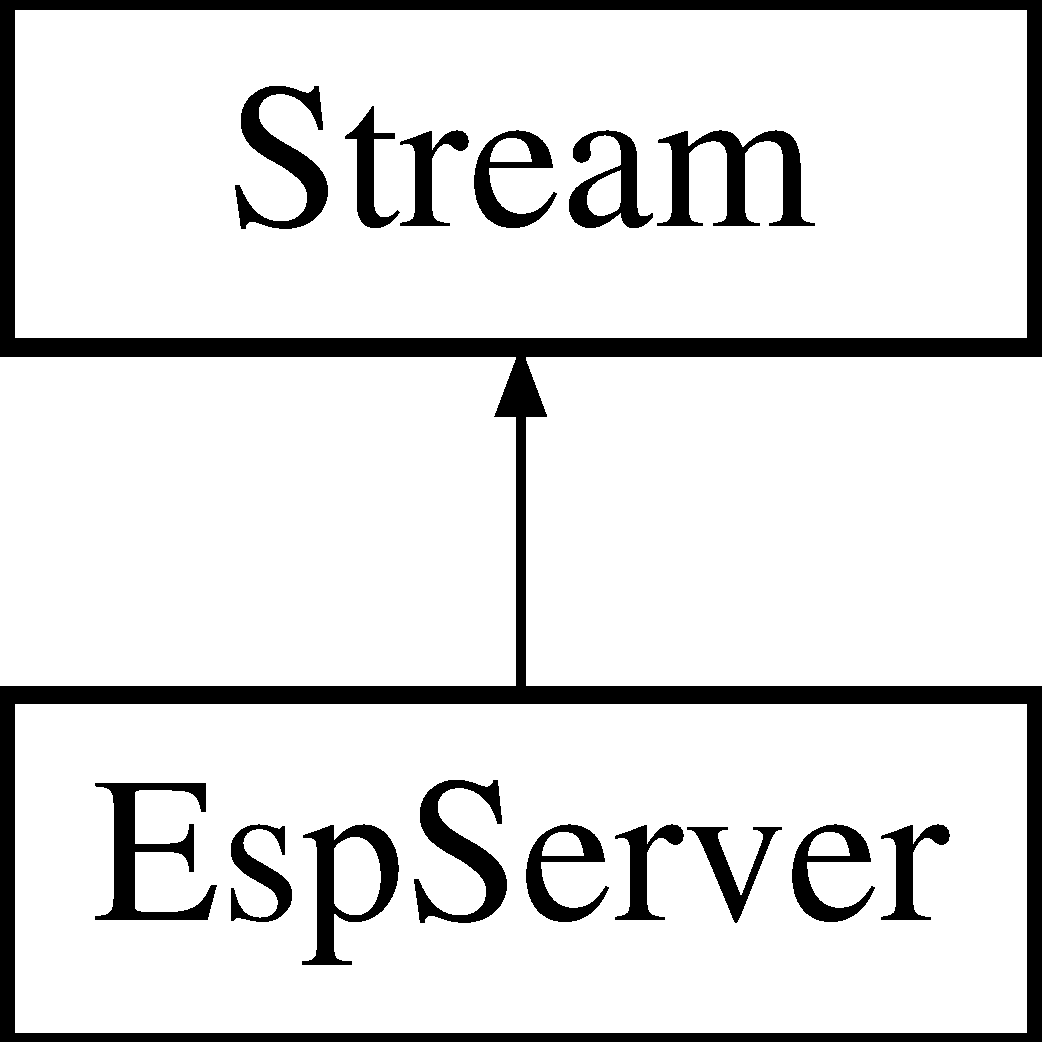
\includegraphics[height=2.000000cm]{class_esp_server}
\end{center}
\end{figure}
\subsection*{Public Member Functions}
\begin{DoxyCompactItemize}
\item 
\mbox{\hyperlink{class_esp_server_aa852bdd3db81410e2b71cafa8adb5c79}{Esp\+Server}} (void)
\item 
void \mbox{\hyperlink{class_esp_server_a1d8682ca0934af03639311e23a71283f}{begin}} (Stream $\ast$esp\+\_\+serial, const char $\ast$ssid, const char $\ast$pass, uint16\+\_\+t port)
\item 
void \mbox{\hyperlink{class_esp_server_a01953c4cc039c37f94dc3e1057126abb}{my\+\_\+ip}} (char $\ast$buf, size\+\_\+t buflen)
\item 
bool \mbox{\hyperlink{class_esp_server_a59fc494d53391b27e2fd75cb750690d9}{connected}} ()
\item 
virtual int \mbox{\hyperlink{class_esp_server_a4549a76725f2e4c013e4d57018366109}{available}} ()
\item 
virtual int \mbox{\hyperlink{class_esp_server_a9040fa1d479d71edf3a826f4691c35c4}{peek}} ()
\item 
virtual int \mbox{\hyperlink{class_esp_server_aaab5dab5b969a87f538242e524431637}{read}} ()
\item 
virtual void \mbox{\hyperlink{class_esp_server_adac116554b543b7c4228c018a85882f5}{flush}} ()
\item 
virtual size\+\_\+t \mbox{\hyperlink{class_esp_server_a7c66fc8d559f4956d4ccea196299bca7}{write}} (const uint8\+\_\+t $\ast$buffer, size\+\_\+t size)
\item 
size\+\_\+t \mbox{\hyperlink{class_esp_server_af32c245c813bbadb566538bba418b0fe}{write}} (uint8\+\_\+t n)
\item 
size\+\_\+t \mbox{\hyperlink{class_esp_server_a0ba52a995edf9b6c2cdf3d396be84ff1}{write}} (unsigned long n)
\item 
size\+\_\+t \mbox{\hyperlink{class_esp_server_a3cfec102ee6f58a2f7e617999ce9f5bb}{write}} (long n)
\item 
size\+\_\+t \mbox{\hyperlink{class_esp_server_a2d9bc6ac05e45a7023be3cd1ca224407}{write}} (unsigned int n)
\item 
size\+\_\+t \mbox{\hyperlink{class_esp_server_a22e7ab55e0aa268cff5b48e763429ec3}{write}} (int n)
\end{DoxyCompactItemize}


\subsection{Constructor \& Destructor Documentation}
\mbox{\Hypertarget{class_esp_server_aa852bdd3db81410e2b71cafa8adb5c79}\label{class_esp_server_aa852bdd3db81410e2b71cafa8adb5c79}} 
\index{Esp\+Server@{Esp\+Server}!Esp\+Server@{Esp\+Server}}
\index{Esp\+Server@{Esp\+Server}!Esp\+Server@{Esp\+Server}}
\subsubsection{\texorpdfstring{Esp\+Server()}{EspServer()}}
{\footnotesize\ttfamily \mbox{\hyperlink{class_esp_server}{Esp\+Server}} (\begin{DoxyParamCaption}\item[{void}]{ }\end{DoxyParamCaption})}



\subsection{Member Function Documentation}
\mbox{\Hypertarget{class_esp_server_a4549a76725f2e4c013e4d57018366109}\label{class_esp_server_a4549a76725f2e4c013e4d57018366109}} 
\index{Esp\+Server@{Esp\+Server}!available@{available}}
\index{available@{available}!Esp\+Server@{Esp\+Server}}
\subsubsection{\texorpdfstring{available()}{available()}}
{\footnotesize\ttfamily int available (\begin{DoxyParamCaption}{ }\end{DoxyParamCaption})\hspace{0.3cm}{\ttfamily [virtual]}}

\mbox{\Hypertarget{class_esp_server_a1d8682ca0934af03639311e23a71283f}\label{class_esp_server_a1d8682ca0934af03639311e23a71283f}} 
\index{Esp\+Server@{Esp\+Server}!begin@{begin}}
\index{begin@{begin}!Esp\+Server@{Esp\+Server}}
\subsubsection{\texorpdfstring{begin()}{begin()}}
{\footnotesize\ttfamily void begin (\begin{DoxyParamCaption}\item[{Stream $\ast$}]{esp\+\_\+serial,  }\item[{const char $\ast$}]{ssid,  }\item[{const char $\ast$}]{pass,  }\item[{uint16\+\_\+t}]{port }\end{DoxyParamCaption})}

\mbox{\Hypertarget{class_esp_server_a59fc494d53391b27e2fd75cb750690d9}\label{class_esp_server_a59fc494d53391b27e2fd75cb750690d9}} 
\index{Esp\+Server@{Esp\+Server}!connected@{connected}}
\index{connected@{connected}!Esp\+Server@{Esp\+Server}}
\subsubsection{\texorpdfstring{connected()}{connected()}}
{\footnotesize\ttfamily bool connected (\begin{DoxyParamCaption}{ }\end{DoxyParamCaption})}

\mbox{\Hypertarget{class_esp_server_adac116554b543b7c4228c018a85882f5}\label{class_esp_server_adac116554b543b7c4228c018a85882f5}} 
\index{Esp\+Server@{Esp\+Server}!flush@{flush}}
\index{flush@{flush}!Esp\+Server@{Esp\+Server}}
\subsubsection{\texorpdfstring{flush()}{flush()}}
{\footnotesize\ttfamily void flush (\begin{DoxyParamCaption}{ }\end{DoxyParamCaption})\hspace{0.3cm}{\ttfamily [virtual]}}

\mbox{\Hypertarget{class_esp_server_a01953c4cc039c37f94dc3e1057126abb}\label{class_esp_server_a01953c4cc039c37f94dc3e1057126abb}} 
\index{Esp\+Server@{Esp\+Server}!my\+\_\+ip@{my\+\_\+ip}}
\index{my\+\_\+ip@{my\+\_\+ip}!Esp\+Server@{Esp\+Server}}
\subsubsection{\texorpdfstring{my\+\_\+ip()}{my\_ip()}}
{\footnotesize\ttfamily void my\+\_\+ip (\begin{DoxyParamCaption}\item[{char $\ast$}]{buf,  }\item[{size\+\_\+t}]{buflen }\end{DoxyParamCaption})}

\mbox{\Hypertarget{class_esp_server_a9040fa1d479d71edf3a826f4691c35c4}\label{class_esp_server_a9040fa1d479d71edf3a826f4691c35c4}} 
\index{Esp\+Server@{Esp\+Server}!peek@{peek}}
\index{peek@{peek}!Esp\+Server@{Esp\+Server}}
\subsubsection{\texorpdfstring{peek()}{peek()}}
{\footnotesize\ttfamily int peek (\begin{DoxyParamCaption}{ }\end{DoxyParamCaption})\hspace{0.3cm}{\ttfamily [virtual]}}

\mbox{\Hypertarget{class_esp_server_aaab5dab5b969a87f538242e524431637}\label{class_esp_server_aaab5dab5b969a87f538242e524431637}} 
\index{Esp\+Server@{Esp\+Server}!read@{read}}
\index{read@{read}!Esp\+Server@{Esp\+Server}}
\subsubsection{\texorpdfstring{read()}{read()}}
{\footnotesize\ttfamily int read (\begin{DoxyParamCaption}{ }\end{DoxyParamCaption})\hspace{0.3cm}{\ttfamily [virtual]}}

\mbox{\Hypertarget{class_esp_server_a7c66fc8d559f4956d4ccea196299bca7}\label{class_esp_server_a7c66fc8d559f4956d4ccea196299bca7}} 
\index{Esp\+Server@{Esp\+Server}!write@{write}}
\index{write@{write}!Esp\+Server@{Esp\+Server}}
\subsubsection{\texorpdfstring{write()}{write()}\hspace{0.1cm}{\footnotesize\ttfamily [1/6]}}
{\footnotesize\ttfamily size\+\_\+t write (\begin{DoxyParamCaption}\item[{const uint8\+\_\+t $\ast$}]{buffer,  }\item[{size\+\_\+t}]{size }\end{DoxyParamCaption})\hspace{0.3cm}{\ttfamily [virtual]}}

\mbox{\Hypertarget{class_esp_server_af32c245c813bbadb566538bba418b0fe}\label{class_esp_server_af32c245c813bbadb566538bba418b0fe}} 
\index{Esp\+Server@{Esp\+Server}!write@{write}}
\index{write@{write}!Esp\+Server@{Esp\+Server}}
\subsubsection{\texorpdfstring{write()}{write()}\hspace{0.1cm}{\footnotesize\ttfamily [2/6]}}
{\footnotesize\ttfamily size\+\_\+t write (\begin{DoxyParamCaption}\item[{uint8\+\_\+t}]{n }\end{DoxyParamCaption})\hspace{0.3cm}{\ttfamily [inline]}}

\mbox{\Hypertarget{class_esp_server_a0ba52a995edf9b6c2cdf3d396be84ff1}\label{class_esp_server_a0ba52a995edf9b6c2cdf3d396be84ff1}} 
\index{Esp\+Server@{Esp\+Server}!write@{write}}
\index{write@{write}!Esp\+Server@{Esp\+Server}}
\subsubsection{\texorpdfstring{write()}{write()}\hspace{0.1cm}{\footnotesize\ttfamily [3/6]}}
{\footnotesize\ttfamily size\+\_\+t write (\begin{DoxyParamCaption}\item[{unsigned long}]{n }\end{DoxyParamCaption})\hspace{0.3cm}{\ttfamily [inline]}}

\mbox{\Hypertarget{class_esp_server_a3cfec102ee6f58a2f7e617999ce9f5bb}\label{class_esp_server_a3cfec102ee6f58a2f7e617999ce9f5bb}} 
\index{Esp\+Server@{Esp\+Server}!write@{write}}
\index{write@{write}!Esp\+Server@{Esp\+Server}}
\subsubsection{\texorpdfstring{write()}{write()}\hspace{0.1cm}{\footnotesize\ttfamily [4/6]}}
{\footnotesize\ttfamily size\+\_\+t write (\begin{DoxyParamCaption}\item[{long}]{n }\end{DoxyParamCaption})\hspace{0.3cm}{\ttfamily [inline]}}

\mbox{\Hypertarget{class_esp_server_a2d9bc6ac05e45a7023be3cd1ca224407}\label{class_esp_server_a2d9bc6ac05e45a7023be3cd1ca224407}} 
\index{Esp\+Server@{Esp\+Server}!write@{write}}
\index{write@{write}!Esp\+Server@{Esp\+Server}}
\subsubsection{\texorpdfstring{write()}{write()}\hspace{0.1cm}{\footnotesize\ttfamily [5/6]}}
{\footnotesize\ttfamily size\+\_\+t write (\begin{DoxyParamCaption}\item[{unsigned int}]{n }\end{DoxyParamCaption})\hspace{0.3cm}{\ttfamily [inline]}}

\mbox{\Hypertarget{class_esp_server_a22e7ab55e0aa268cff5b48e763429ec3}\label{class_esp_server_a22e7ab55e0aa268cff5b48e763429ec3}} 
\index{Esp\+Server@{Esp\+Server}!write@{write}}
\index{write@{write}!Esp\+Server@{Esp\+Server}}
\subsubsection{\texorpdfstring{write()}{write()}\hspace{0.1cm}{\footnotesize\ttfamily [6/6]}}
{\footnotesize\ttfamily size\+\_\+t write (\begin{DoxyParamCaption}\item[{int}]{n }\end{DoxyParamCaption})\hspace{0.3cm}{\ttfamily [inline]}}



The documentation for this class was generated from the following files\+:\begin{DoxyCompactItemize}
\item 
C\+:/\+Users/soere/\+Desktop/\+Projekt Snake/\+Projekt\+\_\+\+Snake/\mbox{\hyperlink{_dumb_server_8h}{Dumb\+Server.\+h}}\item 
C\+:/\+Users/soere/\+Desktop/\+Projekt Snake/\+Projekt\+\_\+\+Snake/\mbox{\hyperlink{_dumb_server_8cpp}{Dumb\+Server.\+cpp}}\end{DoxyCompactItemize}

\hypertarget{class_snake_01_projekt_01auf_01_python_1_1_snake}{}\section{Snake Class Reference}
\label{class_snake_01_projekt_01auf_01_python_1_1_snake}\index{Snake@{Snake}}


\subsection{Detailed Description}
\begin{DoxyVerb}Zusammensezen der Schlange und festlegen des Startpunktes\end{DoxyVerb}
 

The documentation for this class was generated from the following file\+:\begin{DoxyCompactItemize}
\item 
C\+:/\+Users/soere/\+Desktop/\+Projekt Snake/\mbox{\hyperlink{_snake_01_projekt_01auf_01_python_8py}{Snake Projekt auf Python.\+py}}\end{DoxyCompactItemize}

\hypertarget{class_snake_01_projekt_01auf_01_python_1_1_snake__spiel}{}\section{Snake\+\_\+spiel Class Reference}
\label{class_snake_01_projekt_01auf_01_python_1_1_snake__spiel}\index{Snake\+\_\+spiel@{Snake\+\_\+spiel}}
Inheritance diagram for Snake\+\_\+spiel\+:\begin{figure}[H]
\begin{center}
\leavevmode
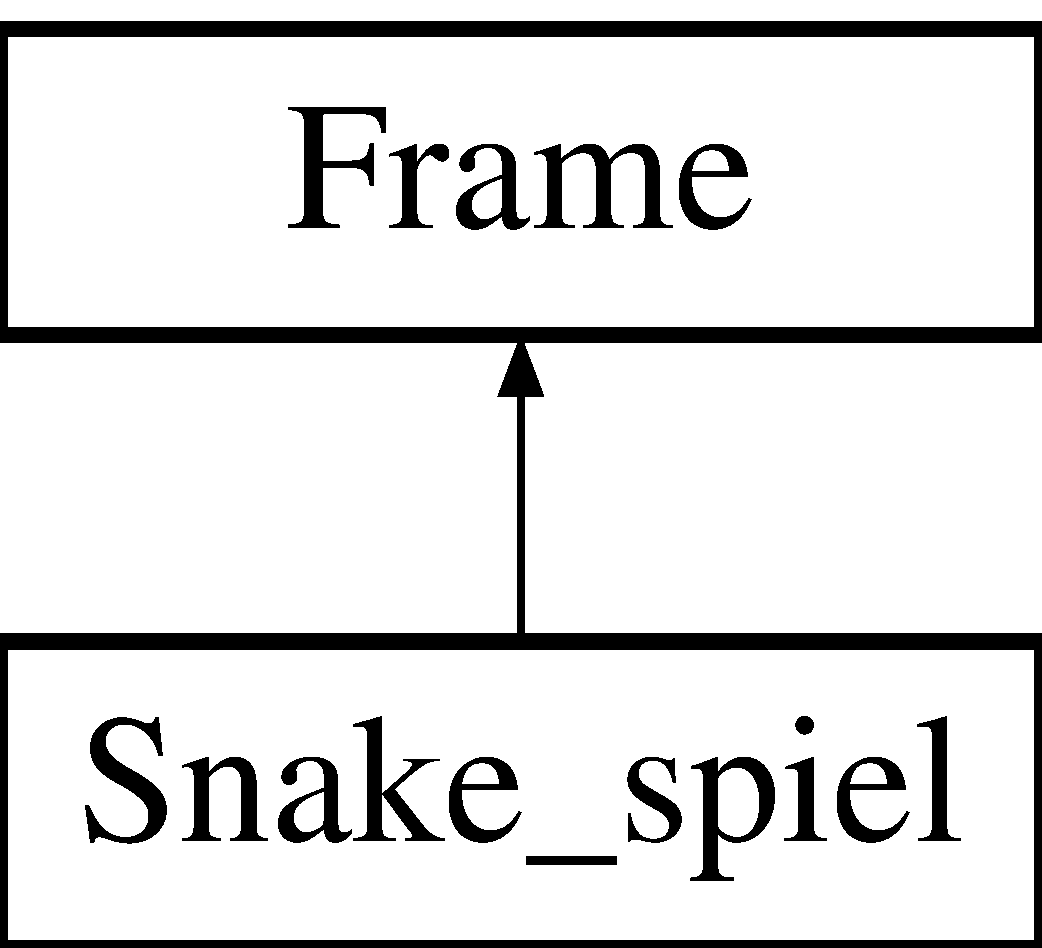
\includegraphics[height=2.000000cm]{class_snake_01_projekt_01auf_01_python_1_1_snake__spiel}
\end{center}
\end{figure}


\subsection{Detailed Description}
\begin{DoxyVerb}Aufbau des GUI\end{DoxyVerb}
 

The documentation for this class was generated from the following file\+:\begin{DoxyCompactItemize}
\item 
C\+:/\+Users/soere/\+Desktop/\+Projekt Snake/\mbox{\hyperlink{_snake_01_projekt_01auf_01_python_8py}{Snake Projekt auf Python.\+py}}\end{DoxyCompactItemize}

\hypertarget{class_snake_01_projekt_01auf_01_python_1_1_snake_k_xC3_xB6rper_st_xC3_xBCck}{}\section{Snake\+Körper\+Stück Class Reference}
\label{class_snake_01_projekt_01auf_01_python_1_1_snake_k_xC3_xB6rper_st_xC3_xBCck}\index{Snake\+Körper\+Stück@{Snake\+Körper\+Stück}}
\subsection*{Public Member Functions}
\begin{DoxyCompactItemize}
\item 
def \mbox{\hyperlink{class_snake_01_projekt_01auf_01_python_1_1_snake_k_xC3_xB6rper_st_xC3_xBCck_a920a2e8c450da87a2461e7913e14cb22}{\+\_\+\+\_\+init\+\_\+\+\_\+}} (self, \mbox{\hyperlink{class_snake_01_projekt_01auf_01_python_1_1_snake_k_xC3_xB6rper_st_xC3_xBCck_a9336ebf25087d91c818ee6e9ec29f8c1}{x}}, \mbox{\hyperlink{class_snake_01_projekt_01auf_01_python_1_1_snake_k_xC3_xB6rper_st_xC3_xBCck_a2fb1c5cf58867b5bbc9a1b145a86f3a0}{y}})
\end{DoxyCompactItemize}
\subsection*{Data Fields}
\begin{DoxyCompactItemize}
\item 
\mbox{\hyperlink{class_snake_01_projekt_01auf_01_python_1_1_snake_k_xC3_xB6rper_st_xC3_xBCck_a9336ebf25087d91c818ee6e9ec29f8c1}{x}}
\item 
\mbox{\hyperlink{class_snake_01_projekt_01auf_01_python_1_1_snake_k_xC3_xB6rper_st_xC3_xBCck_a2fb1c5cf58867b5bbc9a1b145a86f3a0}{y}}
\end{DoxyCompactItemize}


\subsection{Constructor \& Destructor Documentation}
\mbox{\Hypertarget{class_snake_01_projekt_01auf_01_python_1_1_snake_k_xC3_xB6rper_st_xC3_xBCck_a920a2e8c450da87a2461e7913e14cb22}\label{class_snake_01_projekt_01auf_01_python_1_1_snake_k_xC3_xB6rper_st_xC3_xBCck_a920a2e8c450da87a2461e7913e14cb22}} 
\index{Snake Projekt auf Python\+::\+Snake\+Körper\+Stück@{Snake Projekt auf Python\+::\+Snake\+Körper\+Stück}!\+\_\+\+\_\+init\+\_\+\+\_\+@{\+\_\+\+\_\+init\+\_\+\+\_\+}}
\index{\+\_\+\+\_\+init\+\_\+\+\_\+@{\+\_\+\+\_\+init\+\_\+\+\_\+}!Snake Projekt auf Python\+::\+Snake\+Körper\+Stück@{Snake Projekt auf Python\+::\+Snake\+Körper\+Stück}}
\subsubsection{\texorpdfstring{\+\_\+\+\_\+init\+\_\+\+\_\+()}{\_\_init\_\_()}}
{\footnotesize\ttfamily def \+\_\+\+\_\+init\+\_\+\+\_\+ (\begin{DoxyParamCaption}\item[{}]{self,  }\item[{}]{x,  }\item[{}]{y }\end{DoxyParamCaption})}



\subsection{Field Documentation}
\mbox{\Hypertarget{class_snake_01_projekt_01auf_01_python_1_1_snake_k_xC3_xB6rper_st_xC3_xBCck_a9336ebf25087d91c818ee6e9ec29f8c1}\label{class_snake_01_projekt_01auf_01_python_1_1_snake_k_xC3_xB6rper_st_xC3_xBCck_a9336ebf25087d91c818ee6e9ec29f8c1}} 
\index{Snake Projekt auf Python\+::\+Snake\+Körper\+Stück@{Snake Projekt auf Python\+::\+Snake\+Körper\+Stück}!x@{x}}
\index{x@{x}!Snake Projekt auf Python\+::\+Snake\+Körper\+Stück@{Snake Projekt auf Python\+::\+Snake\+Körper\+Stück}}
\subsubsection{\texorpdfstring{x}{x}}
{\footnotesize\ttfamily x}

\mbox{\Hypertarget{class_snake_01_projekt_01auf_01_python_1_1_snake_k_xC3_xB6rper_st_xC3_xBCck_a2fb1c5cf58867b5bbc9a1b145a86f3a0}\label{class_snake_01_projekt_01auf_01_python_1_1_snake_k_xC3_xB6rper_st_xC3_xBCck_a2fb1c5cf58867b5bbc9a1b145a86f3a0}} 
\index{Snake Projekt auf Python\+::\+Snake\+Körper\+Stück@{Snake Projekt auf Python\+::\+Snake\+Körper\+Stück}!y@{y}}
\index{y@{y}!Snake Projekt auf Python\+::\+Snake\+Körper\+Stück@{Snake Projekt auf Python\+::\+Snake\+Körper\+Stück}}
\subsubsection{\texorpdfstring{y}{y}}
{\footnotesize\ttfamily y}



The documentation for this class was generated from the following file\+:\begin{DoxyCompactItemize}
\item 
C\+:/\+Users/soere/\+Desktop/\+Projekt Snake/\mbox{\hyperlink{_snake_01_projekt_01auf_01_python_8py}{Snake Projekt auf Python.\+py}}\end{DoxyCompactItemize}

\hypertarget{class_snake_01_projekt_01auf_01_python_1_1_welt}{}\section{Welt Class Reference}
\label{class_snake_01_projekt_01auf_01_python_1_1_welt}\index{Welt@{Welt}}


\subsection{Detailed Description}
\begin{DoxyVerb}Kreieren der Welt\end{DoxyVerb}
 

The documentation for this class was generated from the following file\+:\begin{DoxyCompactItemize}
\item 
C\+:/\+Users/soere/\+Desktop/\+Projekt Snake/\mbox{\hyperlink{_snake_01_projekt_01auf_01_python_8py}{Snake Projekt auf Python.\+py}}\end{DoxyCompactItemize}

\chapter{File Documentation}
\hypertarget{_dumb_server_8cpp}{}\section{C\+:/\+Users/soere/\+Desktop/\+Projekt Snake/\+Projekt\+\_\+\+Snake/\+Dumb\+Server.cpp File Reference}
\label{_dumb_server_8cpp}\index{C\+:/\+Users/soere/\+Desktop/\+Projekt Snake/\+Projekt\+\_\+\+Snake/\+Dumb\+Server.\+cpp@{C\+:/\+Users/soere/\+Desktop/\+Projekt Snake/\+Projekt\+\_\+\+Snake/\+Dumb\+Server.\+cpp}}
{\ttfamily \#include $<$Arduino.\+h$>$}\newline
{\ttfamily \#include $<$Stream.\+h$>$}\newline
{\ttfamily \#include \char`\"{}Dumb\+Server.\+h\char`\"{}}\newline
\subsection*{Macros}
\begin{DoxyCompactItemize}
\item 
\#define \mbox{\hyperlink{_dumb_server_8cpp_af9850325c242ec48a5d70923c6147de5}{E\+S\+P\+\_\+\+S\+U\+C\+E\+S\+S\+\_\+\+R\+E\+A\+DY}}~((char $\ast$)\char`\"{}ready\textbackslash{}r\textbackslash{}n\char`\"{})
\item 
\#define \mbox{\hyperlink{_dumb_server_8cpp_a62497fcb12b1cedd5fdfbc0755508d87}{E\+S\+P\+\_\+\+S\+U\+C\+E\+S\+S\+\_\+\+OK}}~((char $\ast$)\char`\"{}O\+K\textbackslash{}r\textbackslash{}n\char`\"{})
\item 
\#define \mbox{\hyperlink{_dumb_server_8cpp_a88793823cf689f8ac75d2b9df8e1ca15}{E\+S\+P\+\_\+\+S\+U\+C\+E\+S\+S\+\_\+\+P\+KG}}~((char $\ast$)\char`\"{}+I\+PD,\char`\"{})
\item 
\#define \mbox{\hyperlink{_dumb_server_8cpp_a4a3c8fcc7b628944ea321ad928a00bd9}{E\+S\+P\+\_\+\+S\+U\+C\+E\+S\+S\+\_\+\+I\+PQ}}~((char $\ast$)\char`\"{}+C\+I\+P\+S\+T\+A\+\_\+\+C\+U\+R\+:ip\+:\textbackslash{}\char`\"{}\char`\"{})
\item 
\#define \mbox{\hyperlink{_dumb_server_8cpp_a3df41d167aea12431009366bf32f28b3}{E\+S\+P\+\_\+\+S\+U\+C\+E\+S\+S\+\_\+\+S\+E\+NT}}~((char $\ast$)\char`\"{}S\+E\+ND O\+K\textbackslash{}r\textbackslash{}n\char`\"{})
\end{DoxyCompactItemize}


\subsection{Macro Definition Documentation}
\mbox{\Hypertarget{_dumb_server_8cpp_a4a3c8fcc7b628944ea321ad928a00bd9}\label{_dumb_server_8cpp_a4a3c8fcc7b628944ea321ad928a00bd9}} 
\index{Dumb\+Server.\+cpp@{Dumb\+Server.\+cpp}!E\+S\+P\+\_\+\+S\+U\+C\+E\+S\+S\+\_\+\+I\+PQ@{E\+S\+P\+\_\+\+S\+U\+C\+E\+S\+S\+\_\+\+I\+PQ}}
\index{E\+S\+P\+\_\+\+S\+U\+C\+E\+S\+S\+\_\+\+I\+PQ@{E\+S\+P\+\_\+\+S\+U\+C\+E\+S\+S\+\_\+\+I\+PQ}!Dumb\+Server.\+cpp@{Dumb\+Server.\+cpp}}
\subsubsection{\texorpdfstring{E\+S\+P\+\_\+\+S\+U\+C\+E\+S\+S\+\_\+\+I\+PQ}{ESP\_SUCESS\_IPQ}}
{\footnotesize\ttfamily \#define E\+S\+P\+\_\+\+S\+U\+C\+E\+S\+S\+\_\+\+I\+PQ~((char $\ast$)\char`\"{}+C\+I\+P\+S\+T\+A\+\_\+\+C\+U\+R\+:ip\+:\textbackslash{}\char`\"{}\char`\"{})}

\mbox{\Hypertarget{_dumb_server_8cpp_a62497fcb12b1cedd5fdfbc0755508d87}\label{_dumb_server_8cpp_a62497fcb12b1cedd5fdfbc0755508d87}} 
\index{Dumb\+Server.\+cpp@{Dumb\+Server.\+cpp}!E\+S\+P\+\_\+\+S\+U\+C\+E\+S\+S\+\_\+\+OK@{E\+S\+P\+\_\+\+S\+U\+C\+E\+S\+S\+\_\+\+OK}}
\index{E\+S\+P\+\_\+\+S\+U\+C\+E\+S\+S\+\_\+\+OK@{E\+S\+P\+\_\+\+S\+U\+C\+E\+S\+S\+\_\+\+OK}!Dumb\+Server.\+cpp@{Dumb\+Server.\+cpp}}
\subsubsection{\texorpdfstring{E\+S\+P\+\_\+\+S\+U\+C\+E\+S\+S\+\_\+\+OK}{ESP\_SUCESS\_OK}}
{\footnotesize\ttfamily \#define E\+S\+P\+\_\+\+S\+U\+C\+E\+S\+S\+\_\+\+OK~((char $\ast$)\char`\"{}O\+K\textbackslash{}r\textbackslash{}n\char`\"{})}

\mbox{\Hypertarget{_dumb_server_8cpp_a88793823cf689f8ac75d2b9df8e1ca15}\label{_dumb_server_8cpp_a88793823cf689f8ac75d2b9df8e1ca15}} 
\index{Dumb\+Server.\+cpp@{Dumb\+Server.\+cpp}!E\+S\+P\+\_\+\+S\+U\+C\+E\+S\+S\+\_\+\+P\+KG@{E\+S\+P\+\_\+\+S\+U\+C\+E\+S\+S\+\_\+\+P\+KG}}
\index{E\+S\+P\+\_\+\+S\+U\+C\+E\+S\+S\+\_\+\+P\+KG@{E\+S\+P\+\_\+\+S\+U\+C\+E\+S\+S\+\_\+\+P\+KG}!Dumb\+Server.\+cpp@{Dumb\+Server.\+cpp}}
\subsubsection{\texorpdfstring{E\+S\+P\+\_\+\+S\+U\+C\+E\+S\+S\+\_\+\+P\+KG}{ESP\_SUCESS\_PKG}}
{\footnotesize\ttfamily \#define E\+S\+P\+\_\+\+S\+U\+C\+E\+S\+S\+\_\+\+P\+KG~((char $\ast$)\char`\"{}+I\+PD,\char`\"{})}

\mbox{\Hypertarget{_dumb_server_8cpp_af9850325c242ec48a5d70923c6147de5}\label{_dumb_server_8cpp_af9850325c242ec48a5d70923c6147de5}} 
\index{Dumb\+Server.\+cpp@{Dumb\+Server.\+cpp}!E\+S\+P\+\_\+\+S\+U\+C\+E\+S\+S\+\_\+\+R\+E\+A\+DY@{E\+S\+P\+\_\+\+S\+U\+C\+E\+S\+S\+\_\+\+R\+E\+A\+DY}}
\index{E\+S\+P\+\_\+\+S\+U\+C\+E\+S\+S\+\_\+\+R\+E\+A\+DY@{E\+S\+P\+\_\+\+S\+U\+C\+E\+S\+S\+\_\+\+R\+E\+A\+DY}!Dumb\+Server.\+cpp@{Dumb\+Server.\+cpp}}
\subsubsection{\texorpdfstring{E\+S\+P\+\_\+\+S\+U\+C\+E\+S\+S\+\_\+\+R\+E\+A\+DY}{ESP\_SUCESS\_READY}}
{\footnotesize\ttfamily \#define E\+S\+P\+\_\+\+S\+U\+C\+E\+S\+S\+\_\+\+R\+E\+A\+DY~((char $\ast$)\char`\"{}ready\textbackslash{}r\textbackslash{}n\char`\"{})}

\mbox{\Hypertarget{_dumb_server_8cpp_a3df41d167aea12431009366bf32f28b3}\label{_dumb_server_8cpp_a3df41d167aea12431009366bf32f28b3}} 
\index{Dumb\+Server.\+cpp@{Dumb\+Server.\+cpp}!E\+S\+P\+\_\+\+S\+U\+C\+E\+S\+S\+\_\+\+S\+E\+NT@{E\+S\+P\+\_\+\+S\+U\+C\+E\+S\+S\+\_\+\+S\+E\+NT}}
\index{E\+S\+P\+\_\+\+S\+U\+C\+E\+S\+S\+\_\+\+S\+E\+NT@{E\+S\+P\+\_\+\+S\+U\+C\+E\+S\+S\+\_\+\+S\+E\+NT}!Dumb\+Server.\+cpp@{Dumb\+Server.\+cpp}}
\subsubsection{\texorpdfstring{E\+S\+P\+\_\+\+S\+U\+C\+E\+S\+S\+\_\+\+S\+E\+NT}{ESP\_SUCESS\_SENT}}
{\footnotesize\ttfamily \#define E\+S\+P\+\_\+\+S\+U\+C\+E\+S\+S\+\_\+\+S\+E\+NT~((char $\ast$)\char`\"{}S\+E\+ND O\+K\textbackslash{}r\textbackslash{}n\char`\"{})}


\hypertarget{_dumb_server_8h}{}\section{C\+:/\+Users/soere/\+Desktop/\+Projekt Snake/\+Projekt\+\_\+\+Snake/\+Dumb\+Server.h File Reference}
\label{_dumb_server_8h}\index{C\+:/\+Users/soere/\+Desktop/\+Projekt Snake/\+Projekt\+\_\+\+Snake/\+Dumb\+Server.\+h@{C\+:/\+Users/soere/\+Desktop/\+Projekt Snake/\+Projekt\+\_\+\+Snake/\+Dumb\+Server.\+h}}
{\ttfamily \#include $<$Arduino.\+h$>$}\newline
{\ttfamily \#include $<$Stream.\+h$>$}\newline
\subsection*{Data Structures}
\begin{DoxyCompactItemize}
\item 
class \mbox{\hyperlink{class_esp_server}{Esp\+Server}}
\end{DoxyCompactItemize}

\hypertarget{_snake_01_projekt_01auf_01_python_8py}{}\section{C\+:/\+Users/soere/\+Desktop/\+Projekt Snake/\+Snake Projekt auf Python.\+py File Reference}
\label{_snake_01_projekt_01auf_01_python_8py}\index{C\+:/\+Users/soere/\+Desktop/\+Projekt Snake/\+Snake Projekt auf Python.\+py@{C\+:/\+Users/soere/\+Desktop/\+Projekt Snake/\+Snake Projekt auf Python.\+py}}
\subsection*{Data Structures}
\begin{DoxyCompactItemize}
\item 
class \mbox{\hyperlink{class_snake_01_projekt_01auf_01_python_1_1_arduino}{Arduino}}
\item 
class \mbox{\hyperlink{class_snake_01_projekt_01auf_01_python_1_1_welt}{Welt}}
\item 
class \mbox{\hyperlink{class_snake_01_projekt_01auf_01_python_1_1_snake_k_xC3_xB6rper_st_xC3_xBCck}{Snake\+Körper\+Stück}}
\item 
class \mbox{\hyperlink{class_snake_01_projekt_01auf_01_python_1_1_snake}{Snake}}
\item 
class \mbox{\hyperlink{class_snake_01_projekt_01auf_01_python_1_1_snake__spiel}{Snake\+\_\+spiel}}
\end{DoxyCompactItemize}
\subsection*{Namespaces}
\begin{DoxyCompactItemize}
\item 
 \mbox{\hyperlink{namespace_snake_01_projekt_01auf_01_python}{Snake Projekt auf Python}}
\end{DoxyCompactItemize}
\subsection*{Variables}
\begin{DoxyCompactItemize}
\item 
int \mbox{\hyperlink{namespace_snake_01_projekt_01auf_01_python_a0bb194ef42a009e15b75b9c78234ec82}{W\+E\+L\+T\+\_\+\+G\+RÖ\+S\+SE}} = 500 \char`\"{}\char`\"{}\char`\"{}Allgemeine Spiel Infos\char`\"{}\char`\"{}\char`\"{}
\item 
int \mbox{\hyperlink{namespace_snake_01_projekt_01auf_01_python_a0490a870a678eec59b0e01ade54e7cf5}{Z\+E\+L\+L\+EN}} = 8
\item 
int \mbox{\hyperlink{namespace_snake_01_projekt_01auf_01_python_abfd2595e2773b407f4e4d36545e0d6c2}{S\+N\+A\+K\+E\+T\+E\+M\+PO}} = 200
\item 
\mbox{\hyperlink{namespace_snake_01_projekt_01auf_01_python_a494a6a834239a0d8becd8a87a00ec956}{V\+E\+R\+B\+I\+N\+D\+EN}} = int(input(\char`\"{}Mit Arduino verbinden? Ja(1) Nein(0)\char`\"{}))
\item 
\mbox{\hyperlink{namespace_snake_01_projekt_01auf_01_python_aa798779259654cac04213978cf4297ab}{snake}} = Snake()
\item 
\mbox{\hyperlink{namespace_snake_01_projekt_01auf_01_python_a80417409ca56d97eabc593c02dbb4a1c}{welt}} = Welt(snake)
\item 
\mbox{\hyperlink{namespace_snake_01_projekt_01auf_01_python_a21846080f3e252e582ecd7bf21d38f90}{spiel}} = Snake\+\_\+spiel(welt, snake)
\item 
\mbox{\hyperlink{namespace_snake_01_projekt_01auf_01_python_a9a3afecebf45ad60fdcaa433890500d8}{canv}} = Canvas(spiel.\+master, width=W\+E\+L\+T\+\_\+\+G\+RÖ\+S\+SE, height=W\+E\+L\+T\+\_\+\+G\+RÖ\+S\+SE)
\end{DoxyCompactItemize}

%--- End generated contents ---

% Index
\backmatter
\newpage
\phantomsection
\clearemptydoublepage
\addcontentsline{toc}{chapter}{Index}
\printindex

\end{document}
